% ============================================================
\chapter{System Analysis}
% ============================================================

\section{Data Flow Diagrams / Use Case Diagrams}

NetMind exposes a single actor, the User, who interacts with the system
entirely through one web application rather than a set of separate tools or
commands. Figure~\ref{fig:usecase} shows the use cases reachable from that
entry point, grouped by the mode active at the time of the request. Every use
case in Simulated Mode can change the state of the lab network, while every
use case in Real Network Mode is read-only by design, reflecting the safety
boundary described in Chapter~5: the real-network backend has no capability
that could alter a device outside the Containerlab lab, regardless of how a
request is phrased. Within Simulated Mode, the use cases that change state in
a way that is hard to undo (powering a device off, blocking or allowing a
port, changing a camera's credentials) additionally require the user's
explicit confirmation before they run (Section~\ref{sec:guard}).

\begin{figure}[H]
\centering
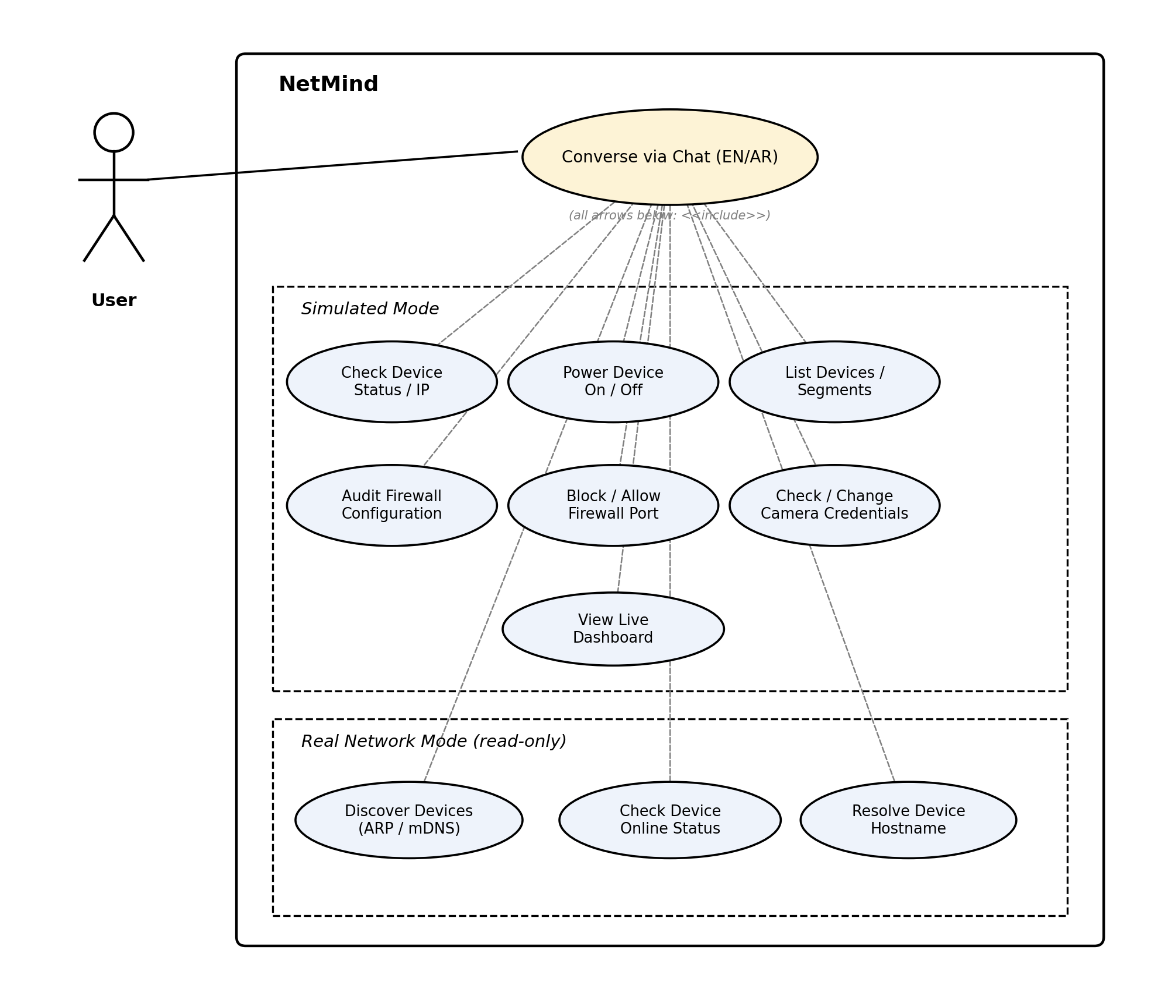
\includegraphics[width=0.78\textwidth]{use-case.png}
\caption{NetMind use case diagram}
\label{fig:usecase}
\end{figure}

\section{System Requirements}

\subsection{Clients, Customer and Users}

NetMind has no external paying customer; it is a Final Year Project built for
academic evaluation, so its requirements are shaped by three groups of
stakeholders. The primary users are the project team members themselves, who
use NetMind daily as network administrators-in-training against the
simulated lab network described in Chapter~5. The direct evaluators are the
project supervisor, Dr.\ Khalil Chebil, and the examining committee, who
assess the system against the functional and non-functional requirements set
out below. Beyond the project itself, NetMind is designed to be usable by any
operator of a small or medium branch network who would rather describe what
they want in natural language than memorise vendor-specific command-line
syntax; such an operator is assumed to have basic networking literacy, such
as knowing what a firewall port or a device IP address is, but not
necessarily fluency in any single configuration language, which is why the
system accepts both Arabic and English.

\subsection{Functional and Data Requirements}

The functional requirements gathered for NetMind are listed in
Table~\ref{tab:fr}.

NetMind's data lives in a small number of well-defined places rather than in
one large database. \code{registry.json}, generated by
\code{build\_registry.py}, is the static-plus-live mapping of each device's
id, owner, type, branch, segment, container name, management IP, and
simulated network IP; it is the single source every tool call resolves a
device name against. Conversation history and the audit log are stored in a
SQLite database (\code{logs/netmind.db}), so a chat session and the record of
every tool call survive a server restart; sessions are still bounded, with a
two-hour idle timeout, a cap of 200 sessions, and at most the system prompt
plus the 40 most recent messages per session. The alert history is kept in
\code{logs/alerts.json}. Device state itself, such as power status, firewall
rules, and camera stream status and credentials, is deliberately not
duplicated anywhere in NetMind: it is read live from Docker and from each
container, with only very short caches, so NetMind's picture cannot drift
from the lab. This removes an entire class of cache-invalidation bugs at the
cost of needing a reachable Docker daemon and live containers for every
query, which is acceptable for a lab environment and is discussed in
Chapter~6.

{\small
\begin{xltabular}{\textwidth}{|p{1.1cm}|Y|}
\hline
\head \textbf{ID} & \textbf{Functional Requirement} \\ \hline
\endhead
FR1 & The system shall allow a user to query the power status and IP address of any registered device by name or owner, tolerating small spelling mistakes in device names. \\ \hline
FR2 & The system shall allow a user to power a device on or off, shall report when the device is already in the requested state rather than performing a redundant action, and shall re-attach a powered-on device to its switch so that it is reachable again. \\ \hline
FR3 & The system shall allow a user to list every registered device, or every device on a specified network segment, validating segment names against the real topology. \\ \hline
FR4 & The system shall allow a user to list a firewall's configured rules, report which ports are open, and audit the firewall for common misconfigurations such as an administrative port left open to any source. Audits and rule listings shall cover both the INPUT chain (traffic to the firewall itself) and the FORWARD chain (traffic passing through it). \\ \hline
FR5 & The system shall allow a user to block or allow a specific port on a firewall. A block or allow shall take effect on both chains, so that it also stops or permits traffic between branches, and the change persists across a normal power cycle. \\ \hline
FR6 & The system shall allow a user to check whether a camera's video stream is reachable, start or stop that stream, and check or change the camera's credentials. \\ \hline
FR7 & In real-network mode, the system shall discover devices on the local network by combining ARP scanning, a ping sweep, IPv6 neighbour discovery and mDNS, and report each device once with its IPv4 address, IPv6 addresses, MAC address, hostname where available, online status and the methods that found it, without altering the state of any discovered device. \\ \hline
FR8 & The system shall accept user requests in either Arabic or English and reply in the same language as the request. \\ \hline
FR9 & The system shall refuse requests that are unrelated to network operations, and shall decline requests that reference a device outside the registry rather than guessing. \\ \hline
FR10 & The web dashboard shall display live device counts, status and open alerts obtained from the same backend state the chat assistant uses, polled at a regular interval, together with a permanent alert history (including when a device comes back online and how long it was down), an activity log of requested and confirmed actions, and a security and reliability report. \\ \hline
FR11 & The system shall not execute a destructive action (power off, block port, allow port, change camera credentials) on the language model's request alone. It shall create a pending action that only the user can confirm or cancel from the interface. \\ \hline
FR12 & Actions on protected devices (the core router and every firewall) shall require an additional explicit acknowledgement. \\ \hline
FR13 & Every tool call, and every confirmed, cancelled or expired destructive action, shall be recorded in an audit log with a timestamp, target, outcome and source. Passwords shall never be written to the log. \\ \hline
FR14 & The system shall allow a user to test whether one lab device can reach another over the simulated data network. \\ \hline
FR15 & The system shall be able to send alert and recovery notifications outside the browser (Telegram), including device, severity and timestamp. \\ \hline
\caption{Functional and data requirements}\label{tab:fr}\\
\end{xltabular}}

\subsection{Non-functional Requirements}

Beyond what NetMind must do, the following qualities were treated as
requirements in their own right, since a network tool that is slow, unsafe,
or hard to set up would not be used regardless of its feature list.

\subsubsection{Usability Requirement}

{\small
\begin{xltabular}{\textwidth}{|p{1.3cm}|Y|}
\hline
\head \textbf{ID} & \textbf{Non-functional Requirement} \\ \hline
\endhead
NFR1 & The system shall provide a single application combining chat and dashboard, requiring no separate manual or training to perform a basic device, firewall, or camera query. \\ \hline
NFR2 & The system shall accept and reply in either Arabic or English, matching the language of the user's request, and shall render structured results such as device or rule lists as formatted tables rather than raw text. \\ \hline
NFR3 & The system shall visually distinguish Simulated Mode from Real Network Mode at all times through an unambiguous, always-visible control. \\ \hline
\caption{Usability requirements}\label{tab:nfr-usability}\\
\end{xltabular}}

\subsubsection{Security Requirement}

{\small
\begin{xltabular}{\textwidth}{|p{1.3cm}|Y|}
\hline
\head \textbf{ID} & \textbf{Non-functional Requirement} \\ \hline
\endhead
NFR4 & Real Network Mode shall be strictly read-only: the real-network backend shall have no capability able to alter the state of any discovered device, enforced in code rather than by the prompt. \\ \hline
NFR5 & Every destructive action available in Simulated Mode, such as powering off a device, blocking or allowing a port, or changing a camera's credentials, shall be confined to the Containerlab lab environment. \\ \hline
NFR6 & The system shall require explicit user confirmation before executing a destructive action, with an additional acknowledgement for protected devices. \textbf{Implemented in Project 1} (Section~\ref{sec:guard}). \\ \hline
NFR12 & (Planned, Project 2) The system shall authenticate users, with roles, before granting access to the web interface. Not yet implemented; stated here as a known, scoped limitation rather than left unaddressed. \\ \hline
NFR13 & The server shall run as a normal user. The only privileges it needs (a raw socket for ARP scanning, and re-attaching a lab device to its bridge) shall be granted narrowly rather than by running the whole server as root. \\ \hline
\caption{Security requirements}\label{tab:nfr-security}\\
\end{xltabular}}

\subsubsection{Performance Requirement}

{\small
\begin{xltabular}{\textwidth}{|p{1.3cm}|Y|}
\hline
\head \textbf{ID} & \textbf{Non-functional Requirement} \\ \hline
\endhead
NFR7 & The agent loop shall cap tool-calling rounds at five per user request, so that no request can loop indefinitely. \\ \hline
NFR8 & The system shall use an LLM inference provider optimised for low response latency, since multi-step tool-calling compounds per-call latency directly into the user's perceived response time. \\ \hline
NFR9 & A real-network scan shall run its discovery methods in parallel, hold the mDNS browse window open for at least six seconds, and reuse a result for 20 seconds, so that repeated questions are answered instantly. \\ \hline
\caption{Performance requirements}\label{tab:nfr-performance}\\
\end{xltabular}}

\subsubsection{Portability Requirement}

{\small
\begin{xltabular}{\textwidth}{|p{1.3cm}|Y|}
\hline
\head \textbf{ID} & \textbf{Non-functional Requirement} \\ \hline
\endhead
NFR10 & The backend shall run on any Linux Docker host with Containerlab installed, including Windows via WSL2 with a native docker-ce installation, and the lab shall be deployable with one command. \\ \hline
NFR11 & The frontend shall require no installation beyond a standard web browser on the machine running NetMind. \\ \hline
\caption{Portability requirements}\label{tab:nfr-portability}\\
\end{xltabular}}

\subsubsection{Reliability Requirement}

{\small
\begin{xltabular}{\textwidth}{|p{1.3cm}|Y|}
\hline
\head \textbf{ID} & \textbf{Non-functional Requirement} \\ \hline
\endhead
NFR14 & Chat sessions, the audit log and the alert history shall survive a server restart. A storage failure shall never break a request. \\ \hline
NFR15 & Every change shall pass automated linting and unit tests, which shall run without Docker, a lab or an API key, before it is merged. \\ \hline
\caption{Reliability requirements}\label{tab:nfr-reliability}\\
\end{xltabular}}
